\section{Definitions}
\label{seq:definitions}

\subsection{Strings}

Throughout this work, let \(\mathcal{A}\) denote a finite ordered alphabet of size \(\alpha =\len{\mathcal{A}}\).

Once we have the source string it is useful to have a special symbol called \emph{sentinel}, which is not from the source's alphabet, but is smaller than the ones from \(\mathcal{A}\). For example, the addition of \emph{sentinel} at the end of the string makes the order on its suffixes strict, since no suffix can then be a prefix of another.
\begin{definition}[Sentinel]
\label{def:sentinel}
    A \emph{sentinel} is some letter \(\$ \notin \mathcal{A}\), smaller than every letter of alphabet \(\mathcal{A}\).
\end{definition}

\subsection{The factorization problem}

Every scheme in this work cuts the source string into consecutive factors and replaces each factor by a reference to already seen part, we call it factorization.
Let us first introduce the factorization of a whole string, that the algorithm has to compute.
\begin{definition}[LZ factorization, \cite{ziv1977}]
\label{def:lz-factorization}
    The \emph{LZ factorization} of \(x\) is the decomposition \(x = w_1 w_2 \cdots w_k\) into nonempty factors such that each \(w_j\) satisfies one of conditions below:
    \begin{enumerate}[label=(\alph*)]
      \item is a letter that does not occur in \(w_1 w_2 \cdots w_{j-1}\),
      \item is the longest substring that occurs at least twice in \(w_1 w_2 \cdots w_j\).
    \end{enumerate}
\end{definition}

\begin{example}[LZ-factorization of string \emph{abaababa}]
\label{ex:lz-factorization}
    Let \(x = abaababa\). Its LZ factorization is
    \[
      x = a \cdot b \cdot a \cdot aba \cdot ba,
    \]
    where \(w_1 = a\) and \(w_2 = b\) are new letters, \(w_3 = a\) is the longest substring occurring twice in \(aba\), \(w_4 = aba\) occurs again at position \(1\), and \(w_5 = ba\) occurs again at position \(2\).
\end{example}

In later implementations we are going to read \Cref{def:lz-factorization} left to right and repeatedly ask the same question in order to form next factor: starting here, how long a factor has already been seen and where, that's why we also need to define such answer, which is pair \((p_i, l_i)\): 

\begin{definition}[Longest previous factor, \cite{kkp2012}]
\label{def:lpf}
    The \emph{longest previous factor} at a position \(i \in \brackets{1 \ldots n}\) is a pair \((p_i, l_i)\) with \(p_i < i\) and
    \[
        x\brackets{p_i \ldots p_i + l_i - 1} = x\brackets{i \ldots i + l_i - 1},
    \]
    and \(l_i > 0\) is as large as possible.
\end{definition}
\noindent Put differently, \(x\brackets{i \ldots i + l_i - 1}\) is the longest prefix of suffix \(i\) that also starts at some earlier position \(p_i\). If \(x\brackets{i}\) is the leftmost occurrence of its letter, no such pair exists, and one sets \(p_i = x\brackets{i}\) and \(l_i = 0\). There may be several fitting \(p_i\) and it does not matter which of them is taken. Longest previous factor array may be computed in \(\bigO(n)\) time (see \cite{kasai2001}).


As extension of previous definition, we need to mention that the factorization can be seen as array of pairs or two arrays that answer the question from before for each position of source string.  
\begin{definition}[\(\mathrm{POS}\) and \(\mathrm{LEN}\) arrays, \cite{chen2008}]
\label{def:pos-len}
    For a position \(i \in \brackets{1, \ldots, n}\), \(\mathrm{LEN}[i]\) is the length of the
    longest factor starting at \(i\) that has an earlier occurrence in \(x\), and
    \(\mathrm{POS}[i]\) is the starting position of one such occurrence, so that
    \[
      x\brackets{\mathrm{POS}[i] \ldots \mathrm{POS}[i] + \mathrm{LEN}[i] - 1}
      = x\brackets{i \ldots i + \mathrm{LEN}[i] - 1},
      \qquad \mathrm{POS}[i] < i .
    \]
    \(\mathrm{LEN}[i] = 0\) and \(\mathrm{POS}[i] = i\) when no such occurrence exists.
\end{definition}

% \[
%     S\pars{i, \; i + \mathrm{LEN}[i] - 1} = S\pars{\mathrm{POS}[i], \; \mathrm{POS}[i] + \mathrm{LEN}[i] - 1} .
% \]
\noindent For visual example we can look at string \(abaababa\). Both arrays \(\mathrm{POS}\) and \(\mathrm{LEN}\) can be filled by hand straight from the description above:
\begin{table}[H]
    \centering
    \begin{tabular}{r|cccccccc}
        \toprule
        \(i\)               & 1 & 2 & 3 & 4 & 5 & 6 & 7 & 8 \\
        \midrule
        \(x[i]\)            & \(a\) & \(b\) & \(a\) & \(a\) & \(b\) & \(a\) & \(b\) & \(a\) \\
        \(\mathrm{LEN}[i]\) & 0 & 0 & 1 & 3 & 2 & 3 & 2 & 1 \\
        \(\mathrm{POS}[i]\) & 1 & 2 & 1 & 1 & 2 & 1 & 2 & 1 \\
        \bottomrule
    \end{tabular}
    \caption{\(\mathrm{POS}\) and \(\mathrm{LEN}\) for \(x = abaababa\).}
    \label{tab:pos-len-example}
\end{table}
\noindent At \(i = 1\) and \(i = 2\) nothing has been seen yet, so \(\mathrm{LEN} = 0\) and the pointer is unused. At \(i = 4\) the factor \(aba\) repeats the prefix \(x[1 \ldots 3]\), and at \(i = 6\) it repeats it again. The pointers listed above happen to be the leftmost occurrences, but the algorithm does not require this, and it may report any earlier one. In this string no factor overlaps its own earlier occurrence, but in general it may: for \(x = aaaa\) we get \(\mathrm{POS}[2] = 1\) and \(\mathrm{LEN}[2] = 3\), so the factor \(x[2 \ldots 4]\) is read from \(x[1 \ldots 3]\), a range it shares three positions with.


\subsection{Index structures}

Computing \((p_i, l_i)\) position by position and comparison by comparison is quadratic. Offline algorithms implemented by us avoid that by sorting the suffixes first: once they are in lexicographical order, suffixes sharing a long prefix stand next to each other, and a repeated factor becomes a contiguous block instead of a search.
\begin{definition}[Suffix array (\(\mathrm{SA}\)), \cite{nong2009}]
\label{def:suffix-array}
    The Suffix Array of \(x\) is an array \([1 \ldots n]\) in which \(\mathrm{SA}[j] = i\) iff
    suffix \(i\) is the \(j\)-th in lexicographical order among all the suffixes of \(x\).
\end{definition}

\begin{table}[H]
    \centering
    \setlength{\tabcolsep}{11pt}
    \renewcommand{\arraystretch}{1.1}
    \begin{tabular}{llcc}
        \toprule
        Year & Authors & Ref & Running time \\
        \midrule
        1972 & Karp, Miller \& Rosenberg & \cite{karp1972} & \(\bigO\pars{n \log n}\) \\
        2003 & K\"arkk\"ainen \& Sanders & \cite{karkkainen2003} & \(\bigO\pars{n}\) \\
        2003 & Ko \& Aluru & \cite{ko2003} & \(\bigO\pars{n}\) \\
        2007 & Larsson \& Sadakane & \cite{larsson2007} & \(\bigO\pars{n \log n}\) \\
        2009 & Nong, Zhang \& Chan & \cite{nong2009} & \(\bigO\pars{n}\) \\
        \bottomrule
    \end{tabular}
    \caption{In \cite{string-algorithms} a handful of algorithms can be found for building suffix array}
    \label{tab:sa-construction}
\end{table}

The structure that holds for each pair of suffixes adjacent in \(\mathrm{SA}\), the length of their common prefix is desirable, since suffix array says in what order the suffixes stand, but not how much two neighbours have in common, what turns adjacency in \(\mathrm{SA}\) into information about repeats of similar prefixes, what in its turn will boil down to the fact that desirable factors are among them. Suffix arrays may be computed in linear time, see \Cref{tab:sa-construction}.
\begin{definition}[Longest Common Prefix Array (\(\mathrm{LCP}\)), \cite{kasai2001}]
\label{def:lcp-array}
    Let \(\mathrm{lcp}(i_1, i_2)\) denote the length of the longest common
    prefix of suffixes \(i_1\) and \(i_2\). The \emph{LCP array} stores the
    longest common prefixes of suffixes adjacent in \(\mathrm{SA}\),
    \[
      \mathrm{LCP}[j] = \mathrm{lcp}(\mathrm{SA}[j-1], \mathrm{SA}[j]),
      \qquad j \in \brackets{2, 3, \ldots, n}
    \]
    with the sentinel values \(\mathrm{LCP}[1] = \mathrm{LCP}[n+1] = -1\).
\end{definition}

Given \(x\) and its suffix array, the \(\mathrm{LCP}\) array can be computed in \(\Theta(n)\) time and \(\bigO(n)\) additional space (\cite{kasai2001}), so having \(\mathrm{SA}\) it costs one linear pass and one more integer array.

\noindent Example of SA and LCP arrays of string \emph{abaababa}:
\begin{table}[H]
    \centering
    \begin{tabular}{r|ccccccccc}
        \toprule
        \(j\)                & 1  & 2 & 3 & 4 & 5 & 6 & 7 & 8 & 9 \\
        \midrule
        \(x[j]\)             & \(a\) & \(b\) & \(a\) & \(a\) & \(b\) & \(a\) & \(b\) & \(a\) & \\
        \(\mathrm{SA}[j]\)   & 8  & 3 & 6 & 1 & 4 & 7 & 2 & 5 & \\
        \(\mathrm{LCP}[j]\)  & \(-1\) & 1 & 1 & 3 & 3 & 0 & 2 & 2 & \(-1\) \\
        \bottomrule
    \end{tabular}
    \caption{\(\mathrm{SA}\) and \(\mathrm{LCP}\) for \(x = abaababa\).}
    \label{tab:sa-lcp-example}
\end{table}

A repeated substring shows up as a block of neighbouring entries of \(\mathrm{SA}\) whose \(\mathrm{LCP}\) are not decreasing, so they share same prefix, and this definition names such a block.
\begin{definition}[Group, \cite{chen2008}]
\label{def:lcp-group}
    For \(l \geq 1\), a \emph{group of level \(l\)} is a maximal range \(\brackets{a \ldots b}\) of \(\mathrm{SA}\) with \(a < b\) such that \(\mathrm{LCP}[j] \geq l\) for all \(j \in \brackets{a+1 \ldots b}\), while \(\mathrm{LCP}[a] < l\) and \(\mathrm{LCP}[b+1] < l\). All suffixes \(\mathrm{SA}[a], \ldots, \mathrm{SA}[b]\) then share a prefix of length \(l\).
\end{definition}

\noindent The groups of \Cref{def:lcp-group} for the same string \emph{abaababa}, read off \Cref{tab:sa-lcp-example}, are as follows:
\begin{table}[H]
    \centering
    \begin{tabular}{ccll}
        \toprule
        range & level & suffixes & common prefix \\
        \midrule
        \([1 \ldots 5]\) & 1     & \(8, 3, 6, 1, 4\) & \(a\) \\
        \([3 \ldots 5]\) & 2, 3  & \(6, 1, 4\)       & \(ab\), \(aba\) \\
        \([6 \ldots 8]\) & 1, 2  & \(7, 2, 5\)       & \(b\), \(ba\) \\
        \bottomrule
    \end{tabular}
    \caption{Groups of \(x = abaababa\).}
    \label{tab:groups}
\end{table}
\noindent Note that \([3 \ldots 5]\) lies inside \([1 \ldots 5]\), and that one range can be a group at several levels at once, where level is length of longest common prefix of these suffixes.
\\

A group gathers candidates for \(p_i\), but it can be large, and scanning it may be costly. The next pair of arrays narrows the search to just two entries. The intuition is that the closer a suffix stands to suffix \(i\) in \(\mathrm{SA}\) the longer the prefix it shares with it, so it is enough to look at the nearest neighbour on each side that starts earlier in the text.
\begin{definition}[Inverse suffix array (\(\mathrm{ISA}\)), \cite{kkp2012}]
\label{def:isa}
    The \emph{inverse suffix array} \(\mathrm{ISA}\) is the inverse permutation of \(\mathrm{SA}\): \(\mathrm{ISA}[i] = j\) iff \(\mathrm{SA}[j] = i\), that is, \(\mathrm{ISA}[i]\) is the position of suffix \(i\) in \(\mathrm{SA}\).
\end{definition}

\begin{definition}[Next and previous smaller values (\(\mathrm{NSV}\) and \(\mathrm{PSV}\)), \cite{kkp2012}]
\label{def:nsv-psv}
    For a position \(i \in 1 \ldots n\) of \(\mathrm{S}\),
    \begin{align*}
        \mathrm{NSV}_{\mathrm{lex}}[i] = \min \set{ j \in [i+1 \ldots n] \mid \mathrm{SA}[j] < \mathrm{SA}[i] }, \\
        \mathrm{PSV}_{\mathrm{lex}}[i] = \max \set{ j \in [1 \ldots i-1] \mid \mathrm{SA}[j] < \mathrm{SA}[i] },
    \end{align*}
    with the value \(0\) when the set is empty. The corresponding positions of the text are
    \begin{align*}
        \mathrm{NSV}[i] = \mathrm{SA}\brackets{ \mathrm{NSV}_{\mathrm{lex}}\brackets{\mathrm{ISA}[i]} },\\
        \mathrm{PSV}[i] = \mathrm{SA}\brackets{ \mathrm{PSV}_{\mathrm{lex}}\brackets{\mathrm{ISA}[i]} },
    \end{align*}
    where we again assume the value \(0\) when the respective index equals \(0\).
\end{definition}

\begin{example}\(\mathrm{NSV}\) and \(\mathrm{PSV}\).]
\label{ex:nsv-psv}
For \(x = abaababa\) with \(\mathrm{SA} = \brackets{8, 3, 6, 1, 4, 7, 2, 5}\) of \Cref{tab:sa-lcp-example}:
    \begin{center}
    \begin{tabular}{r|cccccccc}
        \toprule
        \(i\)                  & 1 & 2 & 3 & 4 & 5 & 6 & 7 & 8 \\
        \midrule
        \(\mathrm{SA}[i]\)     & 8 & 3 & 6 & 1 & 4 & 7 & 2 & 5 \\
        \(\mathrm{ISA}[i]\)    & 4 & 7 & 2 & 5 & 8 & 3 & 6 & 1 \\
        \(\mathrm{PSV}[i]\)    & 0 & 1 & 0 & 1 & 2 & 3 & 4 & 0 \\
        \(\mathrm{NSV}[i]\)    & 0 & 0 & 1 & 2 & 0 & 1 & 2 & 3 \\
        \bottomrule
    \end{tabular}
    \end{center}
    Take, for example, \(i = 6\). Suffix \(6\) sits at \(\mathrm{ISA}[6] = 3\) in \(\mathrm{SA}\), and the neighbouring entries are \(\mathrm{SA}[2] = 3\) on the left and \(\mathrm{SA}[4] = 1\) on the right. Both are smaller than \(6\), so they are the nearest such on each side and \(\mathrm{PSV}[6] = 3\), \(\mathrm{NSV}[6] = 1\). 

    However, for \(i = 1\) both values are \(0\): suffix \(1\) sits at \(\mathrm{ISA}[1] = 4\), and no entry of \(\mathrm{SA}\) on either side of it holds a value smaller than \(1\), as there is none. The same happens at \(i = 3\) on the left and at \(i = 5\) on the right.
\end{example}

The structures of this section offer two ways of arriving at the factorization, and they correspond to the two offline algorithms of this work. One fills the arrays of \Cref{def:pos-len} completely, walking along \(\mathrm{SA}\) and \(\mathrm{LCP}\) and letting every group of \Cref{def:lcp-group} assign its pointers as it closes (\cite{chen2008}). Another computes the pair of \Cref{def:lpf} only at the positions where a factor actually starts, choosing between the two candidates (\cite{kkp2012}). The first computes all \(n\) entries and reads \(k\) of them, the second computes only \(k\) as the factorization proceeds.

\subsection{LZ77 common definitions}

The online setting of \Cref{def:online-problem} has to be made concrete: something must say how much of the already read source the encoder is allowed to keep. In \cite{ziv1977} that role is played by a buffer of fixed length, which slides along the source as factors are emitted.
\begin{definition}[Sliding window, \cite{ziv1977}]
\label{def:sliding-window}
    The encoder keeps a buffer \(B_i\) of \(n\) letters. Its last \(L_s\)
    positions hold the part of the source that has been read but not yet factored;
    the first \(n - L_s\) positions form the \emph{sliding window}, the history
    against which the next word is matched. Once a word of length \(l_i\) has
    been encoded, the buffer is shifted left by \(l_i\) positions and refilled
    with the next \(l_i\) letters of the source:
    \[
      B_{i+1} = B_i(l_i + 1, n)\, S(h_i + 1, h_i + l_i),
    \]
    where \(h_i\) is the position of \(S\) occupied by the last letter of \(B_i\).
\end{definition}

\begin{definition}[Maximal word length (\(L_s\)), \cite{ziv1977}]
\label{def:Ls}
    \(L_s\) is the prescribed upper bound on the length of a source word:
    \(1 \leq l_i \leq L_s\) for every \(i\). It bounds the encoding delay,
    since the encoder never waits for more than \(L_s\) letters before emitting a
    codeword, and it fixes the width of the length field of the codeword.
\end{definition}

\noindent The window bounds how  far back a factor may point to. A second parameter (\(L_s\)) bounds how long it may be, since only fixed amount of last symbols in window are still not processed, they either preserved from last iterations or just were added from source. The two together are what make a codeword of fixed width possible.

\begin{definition}[Codeword length (\(L_c\)), \cite{ziv1977}]
\label{def:Lc}
    Every source word \(S_i\) is mapped to a codeword
    \(C_i = C_{i1} C_{i2} C_{i3}\) over the same alphabet \(\mathcal{A}\), where
    \(C_{i1}\) is the radix-\(\alpha\) representation of the pointer \(p_i - 1\),
    \(C_{i2}\) that of the length \(l_i - 1\), and \(C_{i3}\) is the last letter
    of \(S_i\).
\end{definition}
\noindent All codewords share the fixed length
\[
  L_c = 1 + \ceil{\log_\alpha (n - L_s)} + \ceil{\log_\alpha L_s} 
\]

The online counterpart of \Cref{def:lz-factorization}, stated for the prefix the encoder currently holds instead of the whole source, also fit to bounded on both sides of currently available text in working memory. In algorithm \cite{ziv1977}, since we work on sliding window \(B_{now}\) (see \Cref{def:sliding-window}), the string \(S\) from below is in fact the current buffer \(B_{now}\). 

The rule below is an operation on a string: given a prefix of it, find the longest continuation that starts at some position inside that prefix. The pointer must lie inside the prefix, but the match itself is allowed to run past its end and overlap the continuation being read, so the two ranges may share positions. Such continuation is the next factor of string representation in factorization process with allowed overlapping.
\begin{definition}[Reproducible extension, \cite{ziv1977}]
\label{def:reproducible-extension}
    Let \(S(1,j)\) be a proper prefix of a string \(S\) and let \(i \leq j\).
    Denote by \(L(i)\) the largest nonnegative integer \(l \leq \len{S} - j\)
    such that
    \[
      S(i, i + l - 1) = S(j + 1, j + l),
    \]
    and let \(p\) be a position of \(S(1,j)\) for which
    \(L(p) = \max_{1 \leq i \leq j} L(i)\). The substring
    \(S(j + 1, j + L(p))\) is called the \emph{reproducible extension} of
    \(S(1,j)\) into \(S\), and \(p\) is called the \emph{pointer of the
    reproduction}.
\end{definition}

\subsection{LZ78 common definitions}

LZ78 introduces an alternative referencing scheme. A factor is no longer a substring addressed by position and length, but an entry of a dictionary built dynamically and working on distinct entries. The parsing is therefore arranged so that the entries come out distinct by construction.
\begin{definition}[Incremental parsing, \cite{ziv1978}]
\label{def:incremental-parsing}
    A parsing \(x = y_1 y_2 \cdots y_p\) is \emph{incremental} if the phrases \(y_1, \ldots, y_{p-1}\) are pairwise distinct and, for every \(j\), the word obtained from \(y_j\) by deleting its last letter is either empty or equal to some earlier phrase \(y_i\) with \(i < j\). Writing \(\pi(j) = i\) for that index and \(a_j\) for the deleted letter, every phrase satisfies \(y_j = y_{\pi(j)} a_j\) with \(\pi(j) < j\), where the index \(0\) denotes the empty word. The last phrase \(y_p\) need not be distinct from the earlier ones.
\end{definition}

\begin{example}[Incremental parsing of \emph{abaababa}]
\label{ex:incremental-parsing}
    Let \(x = abaababa\) with the block length \(n = 8\), then the parsing is
    \[
      x = a \cdot b \cdot aa \cdot ba \cdot ba
    \]
\end{example}
\noindent In fact it is easier to follow, once displayed as \emph{trie}, what can be seen below next definition.

Since every phrase extends an earlier one by one letter, the phrases nest as a tree, and finding the next one becomes a walk on it from root down by already met substrings.
\begin{definition}[Dictionary trie, \cite{ziv1978}]
\label{def:dictionary-trie}
    A rooted tree whose edges are labeled by letters of \(\mathcal{A}\), so that the word spelled out on the path from the root to a node is exactly one phrase, and every phrase corresponds to exactly one node. The root is numbered \(0\) and spells the empty word. The node of the \(j\)-th phrase is numbered \(j\). \\
    Let \(\pi\) be a function such that \(\pi(j)\) is the index in their order of creation and refers to the parent of the node \(j\) in trie: \(y_j = y_{\pi(j)} a_j\), the node \(j\) is a child of the node \(\pi(j)\) along the edge labeled \(a_j\), new phrase is inserted as a single new leaf when it emerges.
\end{definition}
Where \(\pi(j)\) is notation for operation taken from \cite{ziv1978}, and it gives the parent node of \(j\). Extending what is described before this definition, we have that the phrases of \Cref{def:incremental-parsing} are stored in a \emph{trie} (see example in \Cref{fig:lz78-trie}.

\noindent
\begin{figure}[H]
    \centering
    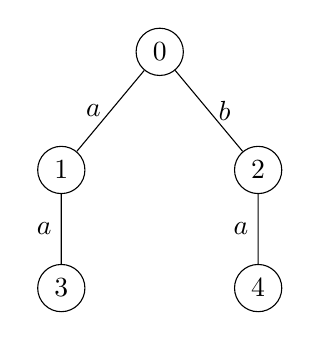
\begin{tikzpicture}[
        level distance=15mm,
        sibling distance=25mm,
        n/.style={draw, circle, minimum size=6mm, inner sep=1pt}
      ]
      \node[n] {\(0\)}
        child { node[n] {\(1\)}
                child { node[n] {\(3\)} edge from parent node[left] {\(a\)} }
                edge from parent node[left] {\(a\)} }
        child { node[n] {\(2\)}
                child { node[n] {\(4\)} edge from parent node[left] {\(a\)} }
                edge from parent node[right] {\(b\)} };
    \end{tikzpicture}
    \caption{The corresponding trie for \(x = abaababa\), with nodes numbered as they emerge. The path from the root to node \(j\) spells the phrase \(y_j\): \(y_1 = a\), \(y_2 = b\), \(y_3 = aa\), \(y_4 = ba\).}
    \label{fig:lz78-trie}
\end{figure}


Since we are going to mention in corresponding chapter the theoretical reasoning behind construction, that the authors provide in LZ78 work (\cite{ziv1978}), we need to add needed definitions, as the compression model here is not stated against other compressors in general but against a fixed class of machines.
\begin{definition}[Finite-state encoder, \cite{ziv1978}]
\label{def:finite-state-encoder}
    A \emph{finite-state encoder} is a quintuple \(E = (Z, A, B, g, f)\), where \(Z\) is a finite set of states, \(\mathcal{A}\) is the input alphabet, \(B\) is a finite set of output words over a binary output alphabet, \(g : Z \times A \to Z\) is the next-state function and \(f : Z \times A \to B\) is the output function. Fed with \(x = x_1 x_2 \cdots\), the encoder emits \(y_i = f(z_i, x_i)\) and moves to \(z_{i+1} = g(z_i, x_i)\), starting from a fixed initial state \(z_1\). The words of \(B\) may have different lengths, and \(B\) may contain the empty word, so block-to-variable and variable-to-variable coding are both covered.
\end{definition}

Information losslessness says nothing about when the input can be recovered: the decoder may have to wait for the whole output before any letter is known. A stronger requirement bounds that waiting time.
\begin{definition}[Information lossless encoder (\(\mathrm{ILE}\)), \cite{ziv1978}]
\label{def:information-lossless}
    An encoder \(E\) is \emph{information lossless} (IL) if for every initial state \(z_1 \in Z\) and every input \(x_1^n \in A^n\) the triple
    \[
        \big(\, z_1, \; f(z_1, x_1^n), \; g(z_1, x_1^n) \,\big)
    \]
    determines \(x_1^n\) uniquely.
\end{definition}

\begin{definition}[Information lossless encoder of finite order (\(\mathrm{ILF}\)), \cite{ziv1978}]
\label{def:ilf}
    An encoder \(E\) is \emph{information lossless of finite order} if there exists a finite positive integer \(m\) such that for every \(z_1 \in Z\) and every \(x_1^m \in A^m\) the pair \((z_1, f(z_1, x_1^m))\) determines the first input letter \(x_1\) uniquely. 
\end{definition}
In other words, an \(\mathrm{ILF}\) encoder can be decoded letter by letter with bounded delay: the letter \(x_1\) is fixed once the output produced for the first \(m\) input letters has arrived, the past being summarized by the known state \(z_1\). This is what a decoder working on the fly needs, and incremental parsing (\Cref{def:incremental-parsing}) provides it: a phrase is emitted as the index of an earlier phrase and one letter, so the decoder recovers it at once by a walk in the trie of \Cref{def:dictionary-trie}, and the delay never exceeds the length of a phrase.
\\

\subsection{Compression ratio}

Three of our four algorithms emit codewords of fixed length over \(\mathcal{A}\), while the encoder of \emph{LZ78} (\cite{ziv1978}) writes a bit stream whose codewords grow with the phrase index. The ratio may be therefore stated in two forms.
\begin{definition}[Compression ratio, \cite{ziv1977}, \cite{ziv1978}]
\label{def:compression-ratio}
    Following \cite{ziv1977}, for a scheme emitting \(N\) codewords of fixed length \(L_c\) over the same alphabet \(\mathcal{A}\) for a source of \(\len{S}\) letters, the \emph{compression ratio} is
    \[
      \rho = \frac{N \cdot L_c}{\len{S}} .
    \]
    Following \cite{ziv1978}, for a scheme emitting an encoded bit stream of total length \(L\) bits, the ratio is measured against the \(\len{S} \log_2 \alpha\) bits needed to write the source,
    \[
      \rho = \frac{L}{\len{S} \log_2 \alpha} .
    \]
\end{definition}

% Used in \Cref{ch:lz78}: it is the bound the encoder is measured against, and unlike the \(h\)-parameters of \Cref{ch:lz77} it belongs to the sequence rather than to a source.
\begin{definition}[Compressibility, \cite{ziv1978}]
\label{def:compressibility}
    Let \(\rho_{E(s)}(x)\) denote the smallest ratio attainable on sequence \(x\) by an information-lossless encoder with at most \(s\) states. The \emph{compressibility} of \(x\) is
    \[
        \rho(x) = \lim_{s \to \infty} \rho_{E(s)}(x) .
    \]
    It is a property of the single sequence \(x\), not attained by any finite-state encoder and approached as the number of states grows.
\end{definition}